%% Causal Protein-Signaling Networks Derived from Multiparameter 
%% Single-Cell Data
%% V1.0
%% 2017/03/23
%% by Ankit Sharma(MT16121) and Divyanshu Srivastava(MT16125)
%%
%% This is a summary of the research paper with an attempt to 
%% highlight the key aspects of the research work done by the authors.

\documentclass[conference]{IEEEtran}

\usepackage{fancyhdr}
\usepackage{graphicx}
\usepackage{float}
\usepackage{amsmath}

\fancypagestyle{firstpage}{
  \fancyhf{}
  \renewcommand{\headrulewidth}{0.4pt}
  \renewcommand{\footrulewidth}{0.4pt}
  \fancyhead[C]{Summary of research article, data set and tentative implementaiton submitted by Ankit Sharma (MT16121) and Divyanshu Srivastava (MT16125) for PGM Project.}
  \fancyfoot[C]{-~\thepage~-}
}
\pagestyle{plain}

\begin{document}

\title{Causal Protein-Signaling Networks Derived from Multiparameter Single-Cell Data}

\author{\IEEEauthorblockN{Karen Sachs}
\and
\IEEEauthorblockN{Omar Perez}
\and
\IEEEauthorblockN{Dana $$Pe'er$$}
\and
\IEEEauthorblockN{Douglas A. Lauffenburger}
\and
\IEEEauthorblockN{Garry P. Nolan}
}

\maketitle

\thispagestyle{firstpage}

\IEEEpeerreviewmaketitle

\section*{Summary of the paper \cite{sachs2005causal}}
 
\subsection{Background Problem}

\subsubsection{Inferring phenotype from genotype}
Genotype is the genetic make-up of an organism and phenotype consists of the traits exhibited as a result of the environmental interaction of the corresponding genotype. Mapping genotype to phenotype has always been a challenge due to the complex nature of the biological networks. Many well known cell signalling networks exhibit cascade effect and as a result molecules may have direct or indirect causal effect on other molecules.

\subsubsection{Selection of computational approach to tackle the problem}
As these molecular signalling pathways are coupled, thus their isolated analysis does not yield accurate results. This issue pitches for the need of a global multivariate approach for simultaneous analysis of coupled signalling networks.
Belief network or Bayesian network is a probabilistic graphical model which is used to study causal relationship among multiple related entities. Several advantages of Bayesian networks like handling stochastic non-linear relationships among entities(molecules in this case) along with their capabilities to handle noise makes them an appropriate choice for the preferred computational approach.

\subsection{Data source and structure estimation from the data}
\subsubsection{Nature of data required for structure estimation}
As Bayesian networks work on the basis of probabilistic approach, therefore a large number of observations are required. Single cell data obtained from  flow cytometry is an optimum choice for the data source.

\subsubsection{Structure estimation from the data source}
Structure estimation involves predicting a graphical model from the data in which the nodes would represent the molecules and the edges would represent the causality flow in between two molecules. The causality can be direct or indirect. The algorithm computes the score corresponding to various graphical models and finally estimates a single structure which is having the best score. The scoring criteria also accounts for a penalty corresponding to the prior over a complex model thereby estimating a structure that is simple as well as accurate.

\subsection{Modelling Bayesian networks with multi variable individual-cell data}
In order to model the bayesian network, single cells were subjected to alterations for which the effect was already known. Nine such perturbations were identified and are listed in Table 1 in the article. Flow cytometry \cite{o2013flow} data was obtained for eleven phosphoproteins and phospholipids corresponding to each cell. Network analysis was done for this data set and estimated structure was obtained.\par
\begin{figure}[H]
\centering
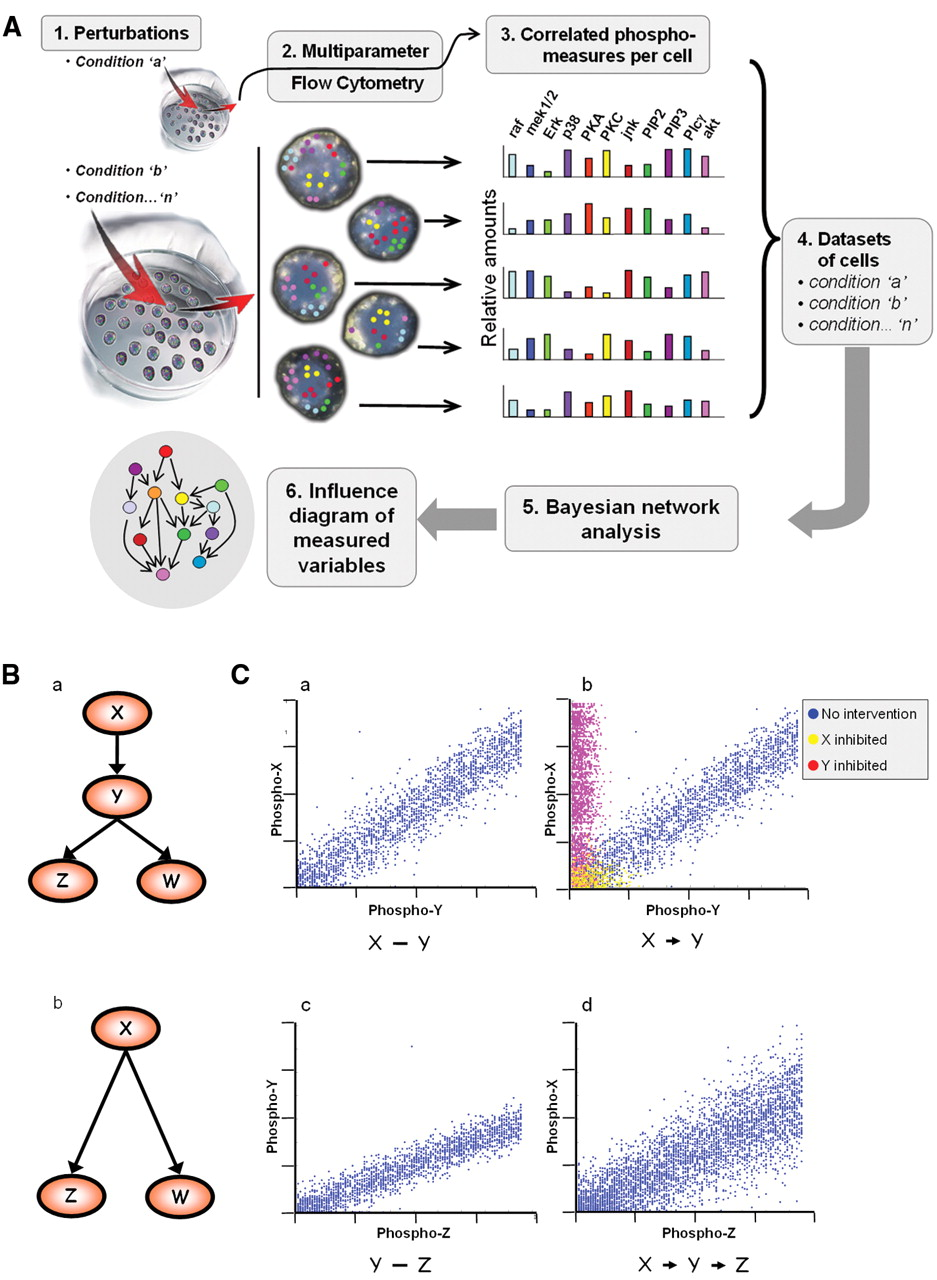
\includegraphics[width=\linewidth]{Images/Fig1.jpg}
\caption{•}
\end{figure}
A simple bayesian network representing four hypothetical proteins (in Fig. 1) was analysed and the inferences were mapped to the various biological phenomena. In Fig 1.B.a molecule X has a causal effect on Y which in turn has causal effects on Z and W. Correlation exists in between X and Y which is illustrated in Fig 1.C.a. In order to determine the direction of influence, flow cytometry data was analysed for inhibited X and it showed that this inhibition affects Y. Whereas inhibition of Y did not had any effect on X as shown in Fig 1.C.b. This implied that causality flows from X to Y. In Fig 1.B.b molecule X has causal effects on Z and W. In this network Y is absent. Though Y is not present in this network but still a noisy correlation was observed between X and Z in Fig 1.C.d. This indicates that Bayesian networks can easily handle hidden variables without the loss of knowledge. This feature is very useful as in biological networks all the intermediates are not always known but still they have an effect on the phenotype.
\par
Also, Bayesian networks omit any redundant edges. For instance the correlation in between X and Z has already been mediated via Y and hence no edge exists from X to Z (Fig 1.B.a). But the statistical correlation of X on Z is independent of observing Y, thus despite the absence of Y, X and Z stand correlated (Fig 1.C.d).

\subsection{A high-accuracy human primary T cell signalling causality map}
The dataset provided along with the article was subjected to Bayesian structure estimation and the arcs/edges were classified as -
\begin{enumerate}
    \item Expected -
    Expected arcs were the ones which were clearly mentioned in the literature to exist. 
    \item Reported -
    Reported arcs were the low confidence arcs that had atleast one literature citation. 
    \item Missing -
    Missing arcs corresponded to the arcs that the estimated structure had missed.
\end{enumerate}

 Total 20 arcs were supposed to exist out of which our structure had 17 (Fig 2.A). All 17 were either reported or expected. 3 arcs were missing which and this happened as Bayesian networks are acyclic in nature and therefore could not capture the feedback loops.
\begin{figure}[h]
\centering
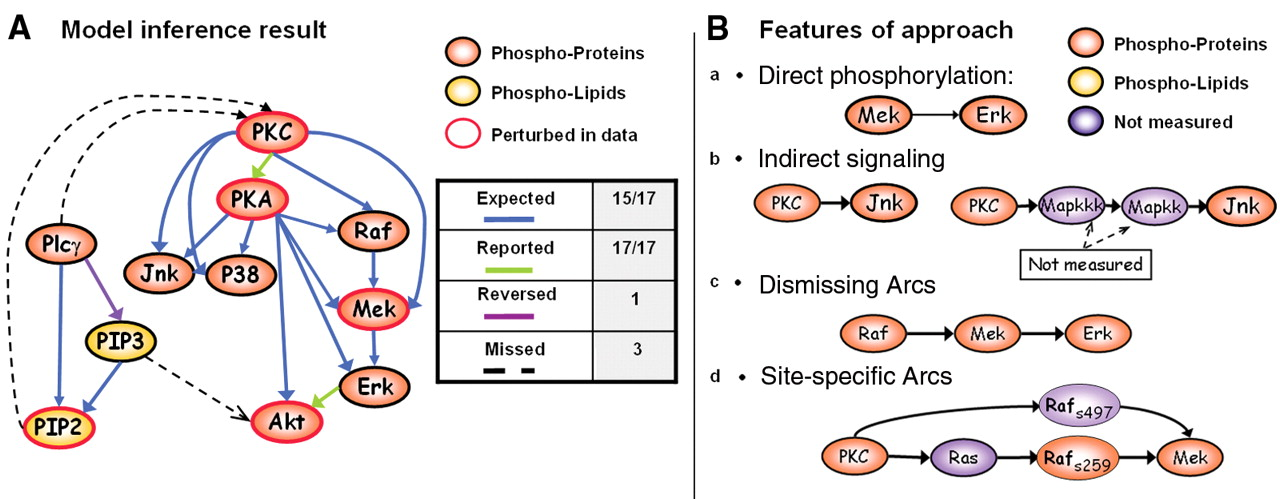
\includegraphics[width=\linewidth]{Images/Fig2.jpg}
\caption{•}
\end{figure}\par
It is clearly evident from the above figure that all the arc direction were correct except for the one arc which was estimated as the reverse of the correct causality direction.\par
Omitting of redundant arcs is illustrated in Fig 2 as no arc exists between Raf and Erk. This is due to existence of arcs Raf-Mek and Mek-Erk. Direct signalling is shown in Fig 2.B.a in which all the proteins are measured. Indirect signalling is shown in Fig 2.B.b in which some of the intermediates are not measured. Bayesian network also captures the arcs corresponding to different sites. For instance, two paths exist from PKC to Mek via different intermediate sites(Raf s497 and Raf s259). As the sites differ thereby these paths do not qualify as redundant paths and hence are represented uniquely (Fig 2.B.d).

\subsection{Experimental confirmation of predicted network causality}
As per the structure (Fig 2), arc PKC-PKA and arc Erk-Akt are the two low confidence arcs due to lack of literature support. The estimated structure was able to infer the correct causality flow for these low confidence arcs. As per the model, alteration of Erk affected Akt whereas vice versa was not true. Similarly, another prediction was made that alteration of Erk should not affect PKA which is also true. Experimental evidence validated the predictions of the probabilistic graph model.

\subsection{Enablers of accurate inference}
The prime reasons for accurate inference were 1.Simultaneous measurement of proteins using flow cytometry 2.Choice of single cell data 3. Use of interventional assays for generating perturbed protein data.\par
Simultaneous measurement of proteins ensured that all correlations were preserved. Choice of single cell data ensured availability of large number of data points required for Bayesian network estimation. Interventional assays generated thousands of data points to analyse proteins after alteration.\par
Further investigation revealed that incorporating all 3 factors led to the most accurate and reliable result (Fig 2).

\subsection*{Discussion}
Various advantages of using Bayesian networks are-\par
\begin{enumerate}
    \item Structure estimation does not require prior knowledge of various paths of the network
    \item The ability to capture direct and indirect influences is beneficial
    \item The networks are robust to hidden variables
\end{enumerate}
Main drawback of Bayesian networks is that the Bayesian networks are acyclic and are unable to capture feedback loops that would make the network cyclic. However, providing time series data would enable Bayesian networks to capture feedback loops.


\noindent\makebox[\linewidth]{\rule{\linewidth}{0.4pt}}
\section*{Summary of the Dataset}
The paper also provides the complete dataset used for the construction of the Bayesian network. The data is organised in 14 .xls files, each of which contains a matrix with 11 columns corresponding to the 11 macromolecules which the paper revolves around. All the entries are their respective expression levels as observed using flow cytometry, briefly explained in the next section. Each row in the matrix corresponds to a single cell, on which the observations are made. There are nearly 800 cells in each file. 14 different files corresponds to 14 different initial stages of the system, whose response in the system are known beforehand. 

\subsection*{Flow Cytometry}
Flow cytometry \cite{o2013flow} is a widely used technique in biotechnology which is used to experimental observe of the internal constituents of a cell or a tissue. The overall idea is to bombard laser at cells and studying the rays passing through them which are detected by a detector. It is used in various types of analysis, but for this study, we limit our self to qualifying bio marker levels.
\newline
This study has used flow cytometry over single cells, which is better than using flow cytometry on bulk cells or at tissue level. At such higher resolutions, cell-to-cell variability is often lost, and thus actual picture withing each cell is not observed. Rather, an average is obtained. For structure estimation, actual values were required, thus single cell resolution study was carried out.
\newline
Each of the .xls file in the data set contains 11 different phosphoprotein and phospholipid levels measured in nearly 800 cells. The values are integers, where a higher value denotes a higher level, or to say that that particular macromolecule is expressed in that cell.

\subsection*{Perturbation in Marker levels}
Each of the 14 different files in the dataset corresponds to 14 different perturbations done in the cells. These perturbations were chosen such that they alter one or more of the macromolecule observed in the cell (based on literature evidences). The perturbations along with their known effects are mentioned in Table 1 of the paper. 

\subsection*{Causality estimation}
Consider figure 2 of the paper suggested that MEK1/2 causes ERK1/2 (also called p44/42). Moreover, on stimulation of the system with a known inhibitor, U0126, MEK levels are known to go down. Because of causality among MEK and ERK, ERK levels are also expected to reduce. These kind of causality relations are expected to be captured while fitting a structure over the provided data. Thus, one can not only estimate correlation among various macromolecules, but the true causality can also be determined. 


\subsection*{Quick Analysis of the dataset on MATLAB \cite{guide1998mathworks}}
In order to have a quick look at the data files, we used MATLAB to import data form all 14 files. We analysed the data in each files individually as well as by combining the entire dataset in one matrix. The entire dataset has entries for 11672 cells, each characterised by 11 different phosphoproteins and phospholipids. 
\par 
Initial findings suggested that the data was log-normal in nature. Consider the histograms for one of the protein, namely ERK 1/2 generated using MATLAB.
\begin{figure}[H]
  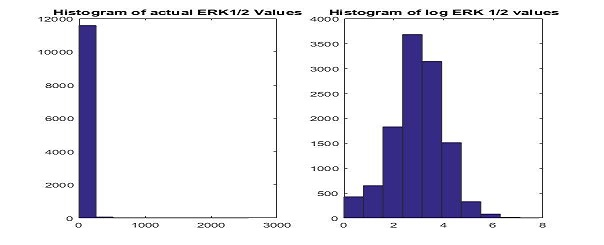
\includegraphics[width=\linewidth]{Images/log-normal.jpg}
  \caption{Histogram of actual and log of ERK1/2 values}
  \label{fig:lognormal}
\end{figure}
Next, we tried to capture the the correlations suggested in the literature. MEK and Raf are shown in the paper to have clear and direct correlation, and a scatter plot among their values directly verified it (see Fig \ref{fig:rafmek}. In the figure, we have also plotted the best fit curve for this data (in orange color).
\begin{figure}[H]
  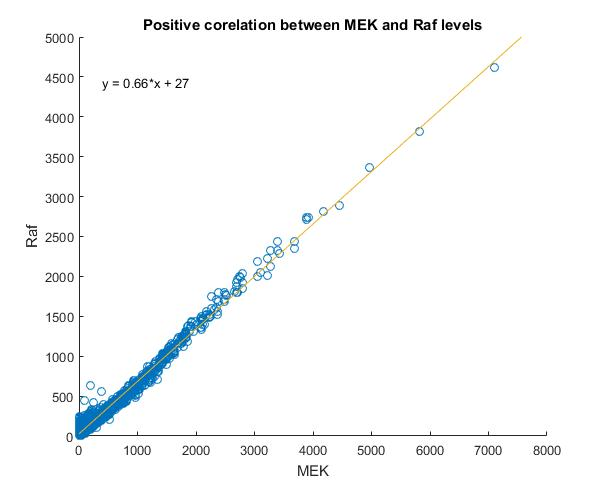
\includegraphics[width=\linewidth]{Images/rafmek.jpg}
  \caption{Correlation Between Raf and MEK levels, figure generated using MATLAB}
  \label{fig:rafmek}
\end{figure}
A similar analysis of ERK and PCL gamma levels was also done. These two were seen to be at a distance in the graph. In the plot too, no such correlation was observed (see Fig. \ref{fig:erkpcl}).
\begin{figure}[H]
  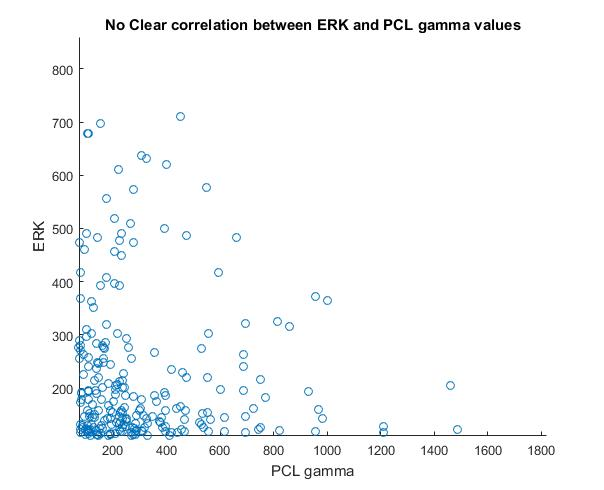
\includegraphics[width=\linewidth]{Images/erkpcl.jpg}
  \caption{Correlation Between ERK and PCL Gamma levels, figure generated using MATLAB}
  \label{fig:erkpcl}
\end{figure}
\par
The dataset clearly has plenty of information in itself, and has a lot to work upon. In the next section we try to propose two approaches in order to estimate a Bayesian structure from the given data.

\noindent\makebox[\linewidth]{\rule{\linewidth}{0.4pt}}

\section*{Proposed Implementation plan}
\textit{The proposed approach is based on our understanding on the topics covered in the class, along with the text books \cite{koller2009probabilistic} and \cite{barber2012bayesian}.}
\par
We would be considering score based structure learning approach to estimate the biological network. The broad idea would be to write a scoring function that would measure the quality of the structure in terms of fitting the data. The highest scoring network would then be considered as the estimated structure for the given data set.\par
We would specifically go for one of the two popular scoring criteria:\par
\begin{itemize}
    \item \textit{Bayesian Information Criterion (BIC) Score}
    \par
    BIC score consists of the likelihood score and the penalty score corresponding to the prior over complex model. The likelihood score would be the absolute score of the model whereas penalty is imposed as due to statistical noise we may encounter over-fitting if the estimated model is fully connected in nature. 
    \[BIC\ Score = MI(x, y) - M(H(x)) - \frac{\log M}{2}Dim[G]\]
    \(M: Total no of samples\\
    I(x, y): Total information between x and y\\
    Dim[G]: Number of independent parameters
    \)
    \\
    The entropy, \(H(x)\) is give by
    \[H(x) = -\sum_{x} \^{p}(x)\log{\^{p}(x)} \]
    \[\^{p}(x) = \frac{M[x]}{M}\]
    Where \(M[x]\) is the number of samples with value of x under consideration.
    \item \textit{Bayesian Dirichlet(BD) Score}
    \par 
    Bayesian Dirichlet score consists of a family score which is a function of the nodes of the networks along with their respective parents.
    \[Family\ Score(x_{i}|\Pi_{i}, \theta)\]\
    where \(\Pi_{i}\) denotes parents of \(x_{i}\) and \(\theta\) is a random variable.
    Also, 
    \[\lim_{M\to\infty} BD\ Score = BIC\ Score \]
\end{itemize}


After finalising the scoring criteria, we would consider an edgeless graph/empty graph. We would be defining the three possible operations to be adding an edge, deleting an edge and reversing the direction of an edge. We would then iteratively perform an operation and would keep on evaluating the score. If the score improves then we would move on to the next operation or else we would discard the last operation that degraded the score. This shall take us through to the optimum structure that would be simple as well as accurate. We expect the estimated structure to be I equivalent to the one given in the paper.\par
After we estimate the structure we will validate it against the correlations that are evident from the data. For instance the correlation between Raf and Mek is easily observable in the scatter plot (Fig 3). This would help us build confidence in the predicted structure.
\par
The obtained results from our approach shall be verified by already available tools like Biolearn \cite{pe2005bayesian}.

\noindent\makebox[\linewidth]{\rule{\linewidth}{0.4pt}}
\medskip
\bibliographystyle{ieeetr}
\bibliography{references}





\end{document}


